% "Isto vai ser um relatório" - Adriano Vinhas

\documentclass{article}
\usepackage[utf8]{inputenc}
\usepackage{graphicx}

\begin{document}

\title{Máquina de calcular \\ Trabalho prático nº1, Computação Adaptativa}
\author{Adriano Vinhas (2009106560, avinhas@student.dei.uc.pt)\\
		José Ribeiro (2008112181, jbaia@student.dei.uc.pt}
\maketitle
\clearpage

% Introdução
\section{Introdução}

Este trabalho, no âmbito da disciplina de Computação Adaptativa, tem como objectivo construir uma rede neuronal capaz de reconhecer digítos (0-9) e operações aritméticas (+,-,=) de modo a ser capaz de servir como uma máquina de calcular.

Este objectivo foi atingido seguindo duas abordagens:
\begin{itemize}
\item Perceptrão
\item Memória Associativa Linear
\end{itemize}

A primeira abordagem é usada para resolver problemas linearmente separáveis e usa funções de activação saturadas. Esta abordagem procura estabelecer uma fronteira de decisão com base nos exemplos que existem para treino. Se existir uma solução possível, o procedimento de treino deverá convergir. Para este trabalho, a função de activação usada no perceptrão é a \texttt{hardlim()}.

A segunda abordagem procura, através de dados de treino que permitam cobrir o maior espaço de procura possível (exemplos que sejam aceitáveis e ao mesmo tempo diferenciáveis entre si), treinar a rede de forma a ser tolerante ao ruído. Desta forma, se na altura de testar a rede surgirem exemplos semelhantes aos protótipos usados no treino, a saída deverá ser semelhante em relação a algum destes protótipos. Deste modo a rede é capaz de recordar os exemplos que foram usados para efectuar o seu treino. Em relação à função de activação, como o próprio nome indica, esta abordagem usa funções de activação lineares.

A parte que foi mais focada na realização deste trabalho foi a construção do dataset, de modo a explorar as situações acima enunciadas. Sumariamente, a construção do dataset foi feita tendo em mente o objectivo de ter diferentes possibilidades de dígitos que fizessem das redes tolerantes a ruído, sem que os erros introduzidos fossem demasiado grandes, inviabilizando assim o bom desempenho destas.

\clearpage

% Treino da rede: Como foi feito o treino para cada um dos casos? Como foi feito o split de dados de validação e de treino?
% Que preocupações foram tidas em conta na hora de conceber o dataset?
\section{A rede neuronal}
Nesta secção estão descritas a arquitectura da rede, já definida pelo professor no enunciado do trabalho, e as preocupações que se tiveram em conta na hora de treinar a rede.

\subsection{Arquitectura}
A arquitectura da rede neuronal usada para o trabalho prático caracteriza-se por 25 entradas, cada uma delas representando uma entrada binária da grelha usada para o preenchimento dos dígitos usando a função \texttt{mpaper()}, e 13 saídas, representando cada uma destas o digíto a ser escolhido.

As figuras~\ref{nn_architecture_perception} e~\ref{nn_architecture_lam} sumariam a arquitectura usada para a abordagem do perceptrão e da memória associativa linear, respectivamente.

\begin{figure}[!h]
  \centering
  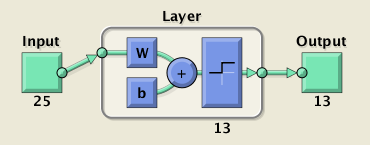
\includegraphics[width=3in]{figures/nn_architecture_perception}
  \caption{Arquitectura da rede neuronal usada no perceptrão para o trabalho prático 1}
  \label{nn_architecture_perception}
  
  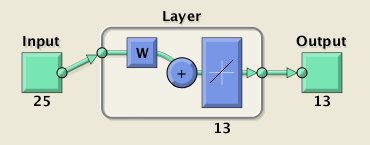
\includegraphics[width=3in]{figures/nn_architecture_lam}
  \caption{Arquitectura da rede neuronal usada na memória associativa linear para o trabalho prático 1}
  \label{nn_architecture_lam}
\end{figure}


\subsection{Treino da rede}
O \textit{dataset} usado para este trabalho é composto por um total de 130 exemplos (10 exemplos para cada um dos 13 dígitos). Deste conjunto, 70\% dos exemplos (de cada dígito) foram usados para treinar a rede, e os restantes 30\% para validação desta e análise de resultados.

De referir que cada um dos conjuntos referidos anteriormente é seleccionado ao acaso, pelo que por cada vez que se corre o processo de constituição dos conjuntos de treino e validação, estes vão ter dígitos diferentes em cada conjunto, tendo como consequência pesos de diferentes valores e redes neuronais de diferentes performances. Para os resultados finais, seleccionou-se a matriz \texttt{W} que, para cada uma das abordagens, maximizava a performance destas.

Para todos os dígitos, procurou-se desenhar pelo menos um \textbf{dígito perfeito}. Os restantes exemplos foram construídos em função do dígito perfeito, introduzindo-se apenas pequenos erros ao modificar uma ou duas entradas ao dígito e criar os vários \textbf{dígitos imperfeitos}.

A figura~\ref{nn_dataset} representa o dataset utilizado para este trabalho.

\begin{figure}[!h]
  \centering
  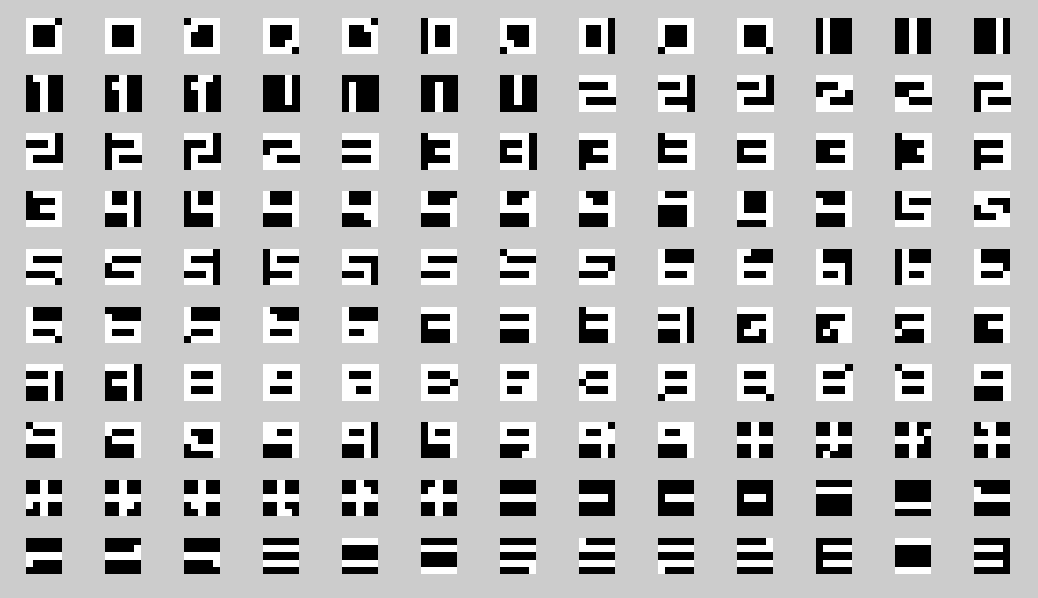
\includegraphics[width=5in]{figures/nn_dataset}
  \caption{Dataset do trabalho prático 1}
  \label{nn_dataset}
\end{figure}

\clearpage

% Gráficos com os resultados. Análise e interpretação.
\section{Resultados e Conclusões}
\indent \indent Nesta secção é feita uma análise de performance às duas abordagens usadas.

De forma a analisar a performance de ambas as abordagens sob diferentes subconjuntos de padrões, 30 subconjuntos distintos de padrões de treino e validação foram gerados. Os erros cometidos na fase de validação por ambas as abordagens quando submetidas ao treino sobre esses subconjuntos foram contabilizados ao longo das 30 execuções. Os resultados obtidos são evidenciados na figura~\ref{nn_long_run_performance}, onde se apresenta a performance média de cada abordagem ao longo das 30 execuções.

\begin{figure}[!h]
  \centering
  \includegraphics[width=5in]{figures/nn_long_run_performance}
  \caption{Performance média das duas abordagens}
  \label{nn_long_run_performance}
\end{figure}

Num total de 1170 classificações\footnote{1170 classificações: 3 classificações por cada um dos 13 dígitos, ao longo de 30 execuções.}, o \textbf{Perceptrão} obteve um total de \textbf{176 classificações incorrectas}, enquanto que a \textbf{Memória Associativa Linear} obteve \textbf{139}; tais resultados correspondem a taxas de eficácia de \textbf{84.96\%} e \textbf{88.12\%}, respectivamente.

A \textbf{Memória Associativa Linear} obteve, assim, uma \textbf{performance média ligeiramente superior} à do Perceptrão na resolução deste problema, considerando os conjuntos de padrões de treino e validação utilizados.

A superioridade de 4\% pode ser justificada pela capacidade de \textbf{tolerância} e \textbf{correcção} de padrões com ruído que um Perceptrão não apresenta; essa capacidade permite que os desvios naturais do dígito protótipo possam ser ignorados de forma a obter, ainda assim, a classificação correcta.

É de notar que a distância de \textit{Hamming} entre os padrões de dígitos perfeitos de símbolos como \texttt{2}, \texttt{5} e \texttt{8} é bastante pequena quando comparada com o número de entradas (tão pequena quanto \textbf{2 entradas diferentes num espaço de 25 entradas}). Tal facto torna o conjunto de dados de treino e validação extremamente importante no que toca à aprendizagem da rede neuronal da relevância e crucialidade de certas entradas para a correcta identificação dos dígitos. É também notório que o \textbf{reduzido espaço de estados} (e consequente proximidade entre dígitos válidos) torna a correcta aprendizagem da rede mais difícil (pelo facto anteriormente mencionado), pelo que julgamos que a classificação beneficiaria de um \textbf{mais alargado conjunto de entradas} (dígitos de 7x5, por exemplo).

\end{document}
